% answers.tex —— 2015 年·福建卷·理科 · 参考答案与详细解析片段
% 由 tools/generate_projects.py 依来源总账自 2015/2015_数学真题_福建理_试题.md + 2015/2015_数学真题_福建理_解析正文.md + 2015/2015_数学真题_福建理_答案要点.md 生成，勿手改（改源 MD 后重跑）


\begin{gktip}
固定 PDF 只含题面，没有答案或评分页。以下解析为本库根据已独立复核题面所作推导，非官方解析；答案要点和本解析稿均已通过独立盲核，正式事实层验收尚未完成。来源发布者、版次、复制链和官方身份未核。
\end{gktip}

\begin{answer}
\gksolhead{1}{复数的幂与集合交集}

\textbf{题目}：

若集合 $A=\{i,i^2,i^3,i^4\}$（$i$ 是虚数单位），$B=\{1,-1\}$，则 $A\cap B=$（　）

\begin{gkopts}(4)
\task （A）$\{-1\}$
\task （B）$\{1\}$
\task （C）$\{1,-1\}$
\task （D）$\varnothing$
\end{gkopts}

\Needspace{4\baselineskip}
\textbf{解析}

\Needspace{5\baselineskip}
由虚数单位的幂循环，
\nopagebreak[4]
\[
i^1=i,\qquad i^2=-1,\qquad i^3=-i,\qquad i^4=1.
\]
因此 $A=\{i,-1,-i,1\}$，与 $B=\{1,-1\}$ 的交集为 $\{1,-1\}$，选 (C)。

\gkanswer{答案：C}

\end{answer}
\begin{answer}
\gksolhead{2}{奇函数}

\textbf{题目}：

下列函数为奇函数的是（　）

\begin{gkopts}(4)
\task （A）$y=\sqrt{x}$
\task （B）$y=|\sin x|$
\task （C）$y=\cos x$
\task （D）$y=e^x-e^{-x}$
\end{gkopts}

\Needspace{4\baselineskip}
\textbf{解析}

\Needspace{5\baselineskip}
对选项 (D) 的函数，
\nopagebreak[4]
\[
f(-x)=e^{-x}-e^x=-(e^x-e^{-x})=-f(x),
\]
故它是奇函数。其余三项分别为偶函数或定义域不关于原点对称，因此选 (D)。

\gkanswer{答案：D}

\end{answer}
\begin{answer}
\gksolhead{3}{双曲线的焦点距离差}

\textbf{题目}：

若双曲线 $E:\dfrac{x^2}{9}-\dfrac{y^2}{16}=1$ 的左、右焦点分别为 $F_1,F_2$，点 $P$ 在双曲线 $E$ 上，且 $|PF_1|=3$，则 $|PF_2|$ 等于（　）

\begin{gkopts}(4)
\task （A）$11$
\task （B）$9$
\task （C）$5$
\task （D）$3$
\end{gkopts}

\Needspace{4\baselineskip}
\textbf{解析}

\Needspace{5\baselineskip}
双曲线的 $a=3$，故双曲线上任一点到两焦点距离之差的绝对值为 $2a=6$：
\nopagebreak[4]
\[
\bigl||PF_1|-|PF_2|\bigr|=6.
\]
令 $d=|PF_2|\geqslant0$。由 $|3-d|=6$ 得代数候选值 $d=9$ 或 $d=-3$；后者与距离非负矛盾，故 $|PF_2|=9$，选 (B)。

\gkanswer{答案：B}

\end{answer}
\begin{answer}
\gksolhead{4}{线性回归}

\textbf{题目}：

为了解某社区居民的家庭年收入与年支出的关系，随机调查了该社区 5 户家庭，得到如下统计数据表：

\begin{center}
\begin{tabular}{lrrrrr}
\toprule
收入 $x$（万元） & 8.2 & 8.6 & 10.0 & 11.3 & 11.9 \\
\midrule
支出 $y$（万元） & 6.2 & 7.5 & 8.0 & 8.5 & 9.8 \\
\bottomrule
\end{tabular}
\end{center}

根据上表可得回归直线方程 $\hat{y}=\hat{b}x+\hat{a}$，其中 $\hat{b}=0.76$，$\hat{a}=\bar{y}-\hat{b}\bar{x}$。据此估计，该社区一户年收入为 15 万元家庭的年支出为（　）

\begin{gkopts}(2)
\task （A）11.4 万元
\task （B）11.8 万元
\task （C）12.0 万元
\task （D）12.2 万元
\end{gkopts}

\Needspace{4\baselineskip}
\textbf{解析}

\Needspace{5\baselineskip}
收入的平均数为
\nopagebreak[4]
\[
\bar{x}=\frac{8.2+8.6+10.0+11.3+11.9}{5}=10,
\]
\Needspace{5\baselineskip}
支出的平均数为
\nopagebreak[4]
\[
\bar{y}=\frac{6.2+7.5+8.0+8.5+9.8}{5}=8.
\]
\Needspace{5\baselineskip}
所以截距 $\hat a=\bar y-0.76\bar x=8-7.6=0.4$。当 $x=15$ 时，
\nopagebreak[4]
\[
\hat y=0.76\times15+0.4=11.8,
\]
估计支出为 $11.8$ 万元，选 (B)。

\gkanswer{答案：B}

\end{answer}
\begin{answer}
\gksolhead{5}{线性规划}

\textbf{题目}：

\Needspace{5\baselineskip}
若变量 $x,y$ 满足约束条件
\nopagebreak[4]
\[
\begin{cases}
x+2y\geqslant0,\\
x-y\leqslant0,\\
x-2y+2\geqslant0,
\end{cases}
\]
则 $z=2x-y$ 的最小值等于（　）

\begin{gkopts}(4)
\task （A）$-\dfrac52$
\task （B）$-2$
\task （C）$-\dfrac32$
\task （D）$2$
\end{gkopts}

\Needspace{4\baselineskip}
\textbf{解析}

\Needspace{5\baselineskip}
约束等价于
\nopagebreak[4]
\[
y\geqslant-\frac{x}{2},\qquad y\geqslant x,\qquad y\leqslant\frac{x}{2}+1.
\]
可行域是三条边界围成的三角形。两条下界相交于 $(0,0)$；$y=x$ 与上界相交于 $(2,2)$；$y=-x/2$ 与上界相交于 $(-1,1/2)$。目标函数 $z=2x-y$ 在三顶点的值分别为 $0,2,-5/2$，故最小值为 $-5/2$，选 (A)。

\gkanswer{答案：B}

\end{answer}
\begin{answer}
\gksolhead{6}{程序框图}

\textbf{题目}：

阅读如图所示的程序框图，运行相应的程序，则输出的结果为（　）

\begin{gkopts}(4)
\task （A）$2$
\task （B）$1$
\task （C）$0$
\task （D）$-1$
\end{gkopts}
\nopagebreak[4]
\begin{center}% Source ID: src-c47985c709ff8ae42e6e192879d604223c58a53c4358056d28f78ad5a9736e3c
% Source PDF SHA-256: a33455d27abdf2c4b344a5b90395bd71269f6fbefdef350375aba074e47ef700
% Source page 1 (printed page 943), question 6. Shape and branch labels follow the fixed page.
\begin{tikzpicture}[
  x=0.82cm,
  y=0.82cm,
  >=stealth,
  every node/.style={font=\small,align=center,inner sep=2pt},
  line width=0.45pt
]
\node[draw,rounded corners=4pt,minimum width=1.75cm,minimum height=0.56cm] (start) at (0,0) {开始};
\node[draw,minimum width=1.45cm,minimum height=0.56cm] (init) at (0,-0.92) {$i=1$};
\node[draw,minimum width=1.55cm,minimum height=0.56cm] (zero) at (0,-1.86) {$S=0$};
\node[draw,minimum width=2.95cm,minimum height=0.82cm] (accumulate) at (0,-3.32)
  {$S=S+\cos\dfrac{i\pi}{2}$};
\node[draw,minimum width=2.05cm,minimum height=0.56cm] (increment) at (0,-4.62) {$i=i+1$};
\node[draw,diamond,aspect=2.6,minimum width=2.6cm,minimum height=0.92cm,inner sep=1pt] (condition) at (0,-5.80) {$i>5?$};
\coordinate (outputtop) at (0,-6.84);
\coordinate (outputbottom) at (0,-7.44);
\draw (-0.88,-6.84)--(-1.12,-7.44)--(0.88,-7.44)--(1.12,-6.84)--cycle;
\node at (0,-7.14) {输出 $S$};
\node[draw,rounded corners=4pt,minimum width=1.75cm,minimum height=0.56cm] (end) at (0,-8.32) {结束};

\draw[->] (start.south)--(init.north);
\draw[->] (init.south)--(zero.north);
\draw[->] (zero.south)--(accumulate.north);
\draw[->] (accumulate.south)--(increment.north);
\draw[->] (increment.south)--(condition.north);
\draw[->] (condition.south)--(outputtop);
\draw[->] (outputbottom)--(end.north);
\draw[->] (condition.west)--(-2.10,-5.80)--(-2.10,-3.32)--(accumulate.west);
\node at (-1.65,-6.08) {否};
\node at (0.42,-6.50) {是};
\end{tikzpicture}
\end{center}
\nopagebreak[4]
\Needspace{4\baselineskip}
\textbf{解析}

\Needspace{5\baselineskip}
程序先令 $i=1,S=0$，每轮先把 $\cos(i\pi/2)$ 加入 $S$，再令 $i$ 增加 $1$，最后判断 $i>5$。因此循环中依次取到 $i=1,2,3,4,5$，累计值为
\nopagebreak[4]
\[
\cos\frac{\pi}{2}+\cos\pi+\cos\frac{3\pi}{2}+\cos2\pi+\cos\frac{5\pi}{2}
=0-1+0+1+0=0.
\]
程序输出 $0$，选 (C)。

\gkanswer{答案：C}

\end{answer}
\begin{answer}
\gksolhead{7}{直线与平面平行的判定}

\textbf{题目}：

若 $l,m$ 是两条不同的直线，$m$ 垂直于平面 $\alpha$，则“$l\perp m$”是“$l\parallel\alpha$”的（　）

（A）充分而不必要条件　（B）必要而不充分条件

（C）充分必要条件　（D）既不充分也不必要条件

\Needspace{4\baselineskip}
\textbf{解析}

因为 $m\perp\alpha$，若 $l\parallel\alpha$，则 $l$ 的方向平行于平面 $\alpha$，所以 $l\perp m$。反过来，$l\perp m$ 只能说明 $l$ 的方向平行于 $\alpha$；按高中立体几何通常定义，$l$ 还可能在 $\alpha$ 内，此时不称为与 $\alpha$ 平行。因此 $l\perp m$ 是 $l\parallel\alpha$ 的必要而不充分条件，选 (B)。

\gkanswer{答案：B}

\end{answer}
\begin{answer}
\gksolhead{8}{根与等差、等比数列}

\textbf{题目}：

若 $a,b$ 是函数 $f(x)=x^2-px+q$（$p>0,q>0$）的两个不同的零点，且 $a,b,-2$ 这三个数可适当排序后成等差数列，也可适当排序后成等比数列，则 $p+q$ 的值等于（　）

\begin{gkopts}(4)
\task （A）$6$
\task （B）$7$
\task （C）$8$
\task （D）$9$
\end{gkopts}

\Needspace{4\baselineskip}
\textbf{解析}

\Needspace{5\baselineskip}
设两个零点为 $a,b$。由韦达定理，
\nopagebreak[4]
\[
a+b=p>0,\qquad ab=q>0.
\]
题设能把 $a,b,-2$ 排成等差数列，因此 $a,b$ 为实数。又由和与积均为正，故 $a,b$ 都为正数。

三个数 $a,b,-2$ 成等比数列时，负数 $-2$ 不可能作为端点，因为等比数列首末两项的乘积等于中项的平方，不能为负。因此 $-2$ 是中项，$ab=(-2)^2=4$。

\Needspace{5\baselineskip}
三个数成等差数列时，按大小排列为 $-2,u,v$，其中 $0<u<v$。中项 $u$ 满足 $u-(-2)=v-u$，即 $v=2u+2$。结合 $uv=4$，
\nopagebreak[4]
\[
u(2u+2)=4 \quad\Longrightarrow\quad (u-1)(u+2)=0.
\]
由于 $u>0$，得 $u=1,v=4$。于是 $p+q=(a+b)+ab=5+4=9$，选 (D)。

\gkanswer{答案：D}

\end{answer}
\begin{answer}
\gksolhead{9}{平面向量与数量积}

\textbf{题目}：

\Needspace{5\baselineskip}
已知 $\overrightarrow{AB}\perp\overrightarrow{AC}$，$|\overrightarrow{AB}|=\dfrac1t$，$|\overrightarrow{AC}|=t$。若点 $P$ 是 $\triangle ABC$ 所在平面内的一点，且
\nopagebreak[4]
\[
\overrightarrow{AP}=\frac{\overrightarrow{AB}}{|\overrightarrow{AB}|}+\frac{4\overrightarrow{AC}}{|\overrightarrow{AC}|},
\]
则 $\overrightarrow{PB}\cdot\overrightarrow{PC}$ 的最大值等于（　）

\begin{gkopts}(4)
\task （A）$13$
\task （B）$15$
\task （C）$19$
\task （D）$21$
\end{gkopts}

\Needspace{4\baselineskip}
\textbf{解析}

\Needspace{5\baselineskip}
取 $A$ 为原点，以 $\overrightarrow{AB}$、$\overrightarrow{AC}$ 的单位向量为两条互相垂直的坐标轴。因 $|\overrightarrow{AB}|=1/t$、$|\overrightarrow{AC}|=t$，可记
\nopagebreak[4]
\[
A=(0,0),\quad B=(1/t,0),\quad C=(0,t).
\]
\Needspace{5\baselineskip}
题设给出 $P=(1,4)$，其中 $t>0$。于是
\nopagebreak[4]
\[
\overrightarrow{PB}=(1/t-1,-4),\qquad
\overrightarrow{PC}=(-1,t-4),
\]
\nopagebreak[4]
\[
\overrightarrow{PB}\cdot\overrightarrow{PC}
=17-4t-\frac1t.
\]
由 $4t+\frac1t\geqslant2\sqrt{4}=4$，等号在 $t=1/2$ 时成立，故最大值为 $13$，选 (A)。

\gkanswer{答案：A}

\end{answer}
\begin{answer}
\gksolhead{10}{导数与函数值比较}

\textbf{题目}：

若定义在 $\mathbb{R}$ 上的函数 $f(x)$ 满足 $f(0)=-1$，其导函数 $f'(x)$ 满足 $f'(x)>k>1$，则下列结论中一定错误的是（　）

（A）$f\!\left(\dfrac1k\right)<\dfrac1k$　（B）$f\!\left(\dfrac1k\right)>\dfrac1{k-1}$

（C）$f\!\left(\dfrac1{k-1}\right)<\dfrac1{k-1}$　（D）$f\!\left(\dfrac1{k-1}\right)>\dfrac{k}{k-1}$

\Needspace{4\baselineskip}
\textbf{解析}

\Needspace{5\baselineskip}
对任意 $x>0$，由拉格朗日中值定理，存在 $\xi\in(0,x)$ 使得
\nopagebreak[4]
\[
f(x)-f(0)=xf'(\xi)>kx.
\]
\Needspace{5\baselineskip}
故 $f(x)>-1+kx$。令 $x=1/(k-1)$，可得
\nopagebreak[4]
\[
f\!\left(\frac1{k-1}\right)>
-1+\frac{k}{k-1}=\frac1{k-1}.
\]
因此选项 (C) 所说的严格小于必定错误。

\gkanswer{答案：C}

\end{answer}
\begin{answer}
\gksolhead{11}{二项式定理}

\textbf{题目}：

$(x+2)^5$ 的展开式中，$x^2$ 的系数等于\gkblank{}。（用数字作答）

\Needspace{4\baselineskip}
\textbf{解析}

\Needspace{5\baselineskip}
$(x+2)^5$ 的 $x^2$ 项来自五个因子中选两个 $x$、三个 $2$，系数为
\nopagebreak[4]
\[
\binom52\,2^3=10\times8=80.
\]

\gkanswer{答案：$80$}

\end{answer}
\begin{answer}
\gksolhead{12}{三角形面积与余弦定理}

\textbf{题目}：

若锐角 $\triangle ABC$ 的面积为 $10\sqrt3$，且 $AB=5$，$AC=8$，则 $BC$ 等于\gkblank{}。

\Needspace{4\baselineskip}
\textbf{解析}

\Needspace{5\baselineskip}
设 $\angle A=\theta$。由面积公式，
\nopagebreak[4]
\[
\frac12\cdot5\cdot8\sin\theta=10\sqrt3,
\]
\Needspace{5\baselineskip}
故 $\sin\theta=\sqrt3/2$。由于三角形为锐角三角形，$\theta=60^\circ$。再用余弦定理，
\nopagebreak[4]
\[
BC^2=5^2+8^2-2\cdot5\cdot8\cos60^\circ=49,
\]
因此 $BC=7$。

\gkanswer{答案：$7$}

\end{answer}
\begin{answer}
\gksolhead{13}{几何概型与定积分}

\textbf{题目}：

如图，点 $A$ 的坐标为 $(1,0)$，点 $C$ 的坐标为 $(2,4)$，函数 $f(x)=x^2$。若在矩形 $ABCD$ 内随机取一点，则此点取自阴影部分的概率等于\gkblank{}。
\nopagebreak[4]
\begin{center}% Source ID: src-c47985c709ff8ae42e6e192879d604223c58a53c4358056d28f78ad5a9736e3c
% Source PDF SHA-256: a33455d27abdf2c4b344a5b90395bd71269f6fbefdef350375aba074e47ef700
% Source page 1 (printed page 943), question 13. Gray fill is the source's shaded set.
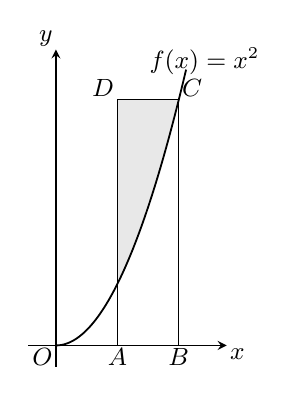
\begin{tikzpicture}[
  x=0.78cm,
  y=0.78cm,
  >=stealth,
  every node/.style={font=\small,inner sep=1pt},
  line width=0.45pt
]
\fill[gray!18] (1,1)--(1,4)--(2,4)
  plot[domain=2:1,samples=60] (\x,{\x*\x})--cycle;

\draw[->] (-0.45,0)--(2.78,0) node[below right] {$x$};
\draw[->] (0,-0.35)--(0,4.82) node[above left] {$y$};
\draw (1,0)--(1,4)--(2,4)--(2,0);
\draw[line width=0.65pt] plot[domain=0:2.12,samples=80] (\x,{\x*\x});

\node[below left] at (0,0) {$O$};
\node[below] at (1,0) {$A$};
\node[below] at (2,0) {$B$};
\node[above left] at (1,4) {$D$};
\node[above right] at (2,4) {$C$};
\node[above right] at (1.47,4.35) {$f(x)=x^2$};
\end{tikzpicture}
\end{center}
\nopagebreak[4]
\Needspace{4\baselineskip}
\textbf{解析}

\Needspace{5\baselineskip}
矩形的顶点为 $A(1,0),B(2,0),C(2,4),D(1,4)$，面积为 $1\times4=4$。图中阴影是在 $1\leqslant x\leqslant2$ 内曲线 $y=x^2$ 上方、直线 $y=4$ 下方的部分，面积为
\nopagebreak[4]
\[
\int_1^2(4-x^2)\,dx
=\left[4x-\frac{x^3}{3}\right]_1^2
=\frac53.
\]
所求概率为阴影面积与矩形面积之比，即 $\dfrac{5/3}{4}=\dfrac5{12}$。

\gkanswer{答案：$\dfrac5{12}$}

\end{answer}
\begin{answer}
\gksolhead{14}{分段函数的值域}

\textbf{题目}：

\Needspace{5\baselineskip}
若函数
\nopagebreak[4]
\[
f(x)=\begin{cases}
-x+6,&x\leqslant2,\\
3+\log_a x,&x>2,
\end{cases}
\]
（$a>0$，且 $a\ne1$）的值域是 $[4,+\infty)$，则实数 $a$ 的取值范围是\gkblank{}。

\Needspace{4\baselineskip}
\textbf{解析}

当 $x\leqslant2$ 时，$-x+6$ 的值域为 $[4,+\infty)$，恰为题设值域。为使第二段不再产生小于 $4$ 的函数值，须有 $3+\log_a x\geqslant4$ 对所有 $x>2$ 成立。

若 $0<a<1$，则 $\log_a x\to-\infty$（$x\to+\infty$），不满足条件。若 $a>1$，$\log_a x$ 随 $x$ 增大，且在 $x>2$ 时其下确界为 $\log_a2$，故需 $\log_a2\geqslant1$，等价于 $1<a\leqslant2$。当 $a=2$ 时第二段值域为 $(4,+\infty)$，与第一段合并仍为 $[4,+\infty)$。所以 $a$ 的取值范围为 $(1,2]$。

\gkanswer{答案：$1<a\leqslant2$}

\end{answer}
\begin{answer}
\gksolhead{15}{二元码的校验方程}

\textbf{题目}：

\Needspace{5\baselineskip}
一个二元码是由 $0$ 和 $1$ 组成的数字串 $x_1x_2\cdots x_n$（$n\in\mathbb{N}^*$），其中 $x_k$（$k=1,2,\cdots,n$）称为第 $k$ 位码元。二元码是通信中常用的码，但在通信过程中有时会发生码元错误（即码元由 $0$ 变为 $1$，或者由 $1$ 变为 $0$）。已知某种二元码 $x_1x_2\cdots x_7$ 的码元满足如下校验方程组：
\nopagebreak[4]
\[
\begin{cases}
x_4\oplus x_5\oplus x_6\oplus x_7=0,\\
x_2\oplus x_3\oplus x_6\oplus x_7=0,\\
x_1\oplus x_3\oplus x_5\oplus x_7=0,
\end{cases}
\]
其中运算 $\oplus$ 定义为：$0\oplus0=0$，$0\oplus1=1$，$1\oplus0=1$，$1\oplus1=0$。现已知一个这种二元码在通信过程中仅在第 $k$ 位发生码元错误后变成了 $1101101$，那么利用上述校验方程组可判定 $k$ 等于\gkblank{}。

\Needspace{4\baselineskip}
\textbf{解析}

\Needspace{5\baselineskip}
收到的码字为 $1101101$。将各校验方程左端依次代入，得到校验结果
\nopagebreak[4]
\[
x_4\oplus x_5\oplus x_6\oplus x_7=1,\qquad
x_2\oplus x_3\oplus x_6\oplus x_7=0,\qquad
x_1\oplus x_3\oplus x_5\oplus x_7=1.
\]
原码满足三式均为 $0$，所以非零校验结果来自那一个错误码元。第 $k$ 位错误会使所有包含 $x_k$ 的校验式翻转。结果 $(1,0,1)$ 只对应第 5 位（它出现在第一、第三式中，不出现在第二式中），故 $k=5$。

\gkanswer{答案：$5$}

\end{answer}
\begin{answer}
\gksolhead{16}{不放回抽取与离散型随机变量}

\textbf{题目}：

某银行规定，一张银行卡若在一天内出现 3 次密码尝试错误，该银行卡将被锁定。小王到该银行取钱时，发现自己忘记了银行卡的密码，但可以确认该银行卡的正确密码是他常用的 6 个密码之一，小王决定从中不重复地随机选择 1 个进行尝试。若密码正确，则结束尝试；否则继续尝试，直至该银行卡被锁定。

(1) 求当天小王的该银行卡被锁定的概率；

(2) 设当天小王用该银行卡尝试密码的次数为 $X$，求 $X$ 的分布列和数学期望。

\Needspace{4\baselineskip}
\textbf{解析}

\gksubpart{(1)}

\Needspace{5\baselineskip}
正确密码在随机排列的六个候选密码中的位置等可能为 $1,2,\ldots,6$。若它在前三位，小王在密码正确时停止；若位置在第 4 至第 6 位，前三次均错，银行卡被锁定。因此锁卡概率为
\nopagebreak[4]
\[
\frac{3}{6}=\frac12.
\]

\gksubpart{(2)}

\Needspace{5\baselineskip}
若正确密码在第 3 位，小王第三次恰好猜中；若在第 4 至第 6 位，第三次错误后银行卡被锁。这四种位置都对应 $X=3$。因此尝试次数 $X$ 的分布为
\nopagebreak[4]
\[
P(X=1)=\frac16,\qquad P(X=2)=\frac16,\qquad P(X=3)=\frac46=\frac23.
\]
\Needspace{5\baselineskip}
于是
\nopagebreak[4]
\[
E(X)=1\cdot\frac16+2\cdot\frac16+3\cdot\frac23=\frac52.
\]

\gkanswer{答案（1）：$\dfrac12$。}

\gkanswer{答案（2）：$P(X=1)=\dfrac16$，$P(X=2)=\dfrac16$，$P(X=3)=\dfrac23$；数学期望 $E(X)=\dfrac52$。}

\end{answer}
\begin{answer}
\gksolhead{17}{空间向量与二面角}

\textbf{题目}：

如图，在几何体 $ABCDE$ 中，四边形 $ABCD$ 是矩形，$AB\perp$ 平面 $BEC$，$BE\perp EC$，$AB=BE=EC=2$，$G,F$ 分别是线段 $BE,DC$ 的中点。

(1) 求证：$GF\parallel$ 平面 $ADE$；

(2) 求平面 $AEF$ 与平面 $BEC$ 所成锐二面角的余弦值。
\nopagebreak[4]
\begin{center}% Source ID: src-c47985c709ff8ae42e6e192879d604223c58a53c4358056d28f78ad5a9736e3c
% Source PDF SHA-256: a33455d27abdf2c4b344a5b90395bd71269f6fbefdef350375aba074e47ef700
% Source page 1 (printed page 943), question 17. Hidden edges and auxiliary segments follow the fixed page.
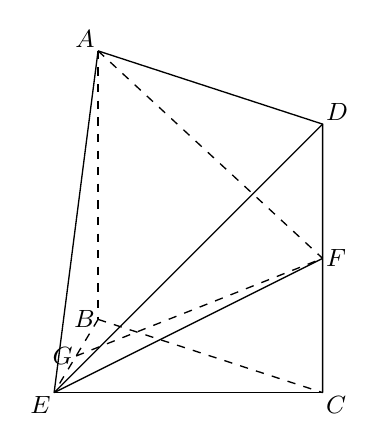
\begin{tikzpicture}[
  x=0.62cm,
  y=0.62cm,
  every node/.style={font=\small,inner sep=1pt},
  line width=0.48pt
]
\coordinate (A) at (0.9,7.0);
\coordinate (B) at (0.9,1.5);
\coordinate (C) at (5.5,0);
\coordinate (D) at (5.5,5.5);
\coordinate (E) at (0,0);
\coordinate (F) at (5.5,2.75);
\coordinate (G) at (0.45,0.75);

% Visible outline and construction segments.
\draw (A)--(D)--(C);
\draw (E)--(A);
\draw (E)--(C);
\draw (E)--(D);
\draw (E)--(F);
\draw[dashed] (A)--(B);
\draw[dashed] (B)--(C);
\draw[dashed] (B)--(E);
\draw[dashed] (A)--(F);
\draw[dashed] (G)--(F);

\node[above left] at (A) {$A$};
\node[left] at (B) {$B$};
\node[below right] at (C) {$C$};
\node[above right] at (D) {$D$};
\node[below left] at (E) {$E$};
\node[right] at (F) {$F$};
\node[left] at (G) {$G$};
\end{tikzpicture}
\end{center}
\nopagebreak[4]
\Needspace{4\baselineskip}
\textbf{解析}

\Needspace{5\baselineskip}
建立直角坐标系，使 $E=(0,0,0)$，$B=(2,0,0)$，$C=(0,2,0)$。因 $AB\perp$ 平面 $BEC$ 且 $AB=2$，可取 $A=(2,0,2)$；矩形 $ABCD$ 给出 $D=(0,2,2)$。从而
\nopagebreak[4]
\[
G=(1,0,0),\qquad F=(0,2,1).
\]

\gksubpart{(1)}

\Needspace{5\baselineskip}
平面 $ADE$ 过原点，方向向量可取
\nopagebreak[4]
\[
\overrightarrow{EA}=(2,0,2),\qquad \overrightarrow{ED}=(0,2,2).
\]
\Needspace{5\baselineskip}
其法向量可取 $\boldsymbol n=(1,1,-1)$，故平面方程为 $x+y-z=0$。又
\nopagebreak[4]
\[
\overrightarrow{GF}=(-1,2,1),\qquad
\boldsymbol n\cdot\overrightarrow{GF}=-1+2-1=0.
\]
所以直线 $GF$ 的方向平行于平面 $ADE$；而 $G$ 不在该平面内，因为 $1+0-0\ne0$。因此 $GF\parallel$ 平面 $ADE$。

\gksubpart{(2)}

\Needspace{5\baselineskip}
平面 $BEC$ 为 $z=0$，法向量为 $\boldsymbol n_1=(0,0,1)$。平面 $AEF$ 的两个方向向量为
\nopagebreak[4]
\[
\overrightarrow{EA}=(2,0,2),\qquad \overrightarrow{EF}=(0,2,1),
\]
\Needspace{5\baselineskip}
故法向量可取
\nopagebreak[4]
\[
\boldsymbol n_2=\overrightarrow{EA}\times\overrightarrow{EF}=(-4,-2,4).
\]
\Needspace{5\baselineskip}
两平面所成锐二面角的余弦为
\nopagebreak[4]
\[
\frac{|\boldsymbol n_1\cdot\boldsymbol n_2|}
{|\boldsymbol n_1|\,|\boldsymbol n_2|}
=\frac4{\sqrt{36}}=\frac23.
\]

\gkanswer{答案（1）：结论成立，$GF\parallel$ 平面 $ADE$。}

\gkanswer{答案（2）：$\dfrac23$。}

\end{answer}
\begin{answer}
\gksolhead{18}{椭圆与以弦为直径的圆}

\textbf{题目}：

已知椭圆 $E:\dfrac{x^2}{a^2}+\dfrac{y^2}{b^2}=1$（$a>b>0$）过点 $(0,\sqrt2)$，且离心率 $e=\dfrac{\sqrt2}{2}$。

(1) 求椭圆 $E$ 的方程；

(2) 设直线 $l:x=my-1$（$m\in\mathbb{R}$）交椭圆 $E$ 于 $A,B$ 两点，判断点 $G\!\left(-\dfrac94,0\right)$ 与以线段 $AB$ 为直径的圆的位置关系，并说明理由。
\nopagebreak[4]
\begin{center}% Source ID: src-c47985c709ff8ae42e6e192879d604223c58a53c4358056d28f78ad5a9736e3c
% Source PDF SHA-256: a33455d27abdf2c4b344a5b90395bd71269f6fbefdef350375aba074e47ef700
% Source page 2 (printed page 944), question 18. Axes, ellipse, secant, and point G follow the fixed page.
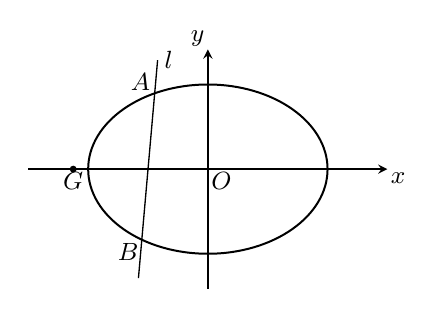
\begin{tikzpicture}[
  x=0.76cm,
  y=0.76cm,
  >=stealth,
  every node/.style={font=\small,inner sep=1pt},
  line width=0.48pt
]
\draw[line width=0.72pt] (0,0) ellipse [x radius=2,y radius=1.4142];
\draw[->] (-3.0,0)--(3.0,0) node[below right] {$x$};
\draw[->] (0,-2.0)--(0,2.0) node[above left] {$y$};
\draw (-1.16,-1.82)--(-0.84,1.82);
\fill (-2.25,0) circle (1.25pt);

\node[above left] at (-0.91,1.26) {$A$};
\node[below left] at (-1.10,-1.18) {$B$};
\node[above right] at (-0.78,1.62) {$l$};
\node[below right] at (0,0) {$O$};
\node[below] at (-2.25,0) {$G$};
\end{tikzpicture}
\end{center}
\nopagebreak[4]
\Needspace{4\baselineskip}
\textbf{解析}

\gksubpart{(1)}

\Needspace{5\baselineskip}
椭圆经过 $(0,\sqrt2)$，故 $b^2=2$。又
\nopagebreak[4]
\[
e^2=1-\frac{b^2}{a^2}=\frac12,
\]
\Needspace{5\baselineskip}
因此 $a^2=4$，椭圆方程为
\nopagebreak[4]
\[
\frac{x^2}{4}+\frac{y^2}{2}=1.
\]

\gksubpart{(2)}

\Needspace{5\baselineskip}
把直线 $x=my-1$ 参数化为 $(x,y)=(mt-1,t)$。交点 $A,B$ 对应参数 $t_1,t_2$，它们满足
\nopagebreak[4]
\[
\frac{(mt-1)^2}{4}+\frac{t^2}{2}=1
\quad\Longleftrightarrow\quad
(m^2+2)t^2-2mt-3=0.
\]
\Needspace{5\baselineskip}
由韦达定理，
\nopagebreak[4]
\[
t_1+t_2=\frac{2m}{m^2+2},\qquad
t_1t_2=-\frac3{m^2+2}.
\]
以 $AB$ 为直径的圆，其上点 $X$ 满足
\Needspace{5\baselineskip}
$(\overrightarrow{XA}\cdot\overrightarrow{XB})=0$；当该数量积为正时，$X$ 在圆外。对 $G=(-9/4,0)$，利用 $x_i=mt_i-1$ 计算得
\nopagebreak[4]
\[
\overrightarrow{GA}\cdot\overrightarrow{GB}
=\left(-\frac54-mt_1\right)\left(-\frac54-mt_2\right)+t_1t_2
=\frac{17m^2+2}{16(m^2+2)}>0.
\]
该式对所有实数 $m$ 均为正，因此 $G$ 始终在以 $AB$ 为直径的圆外。

\gkanswer{答案（1）：$\dfrac{x^2}{4}+\dfrac{y^2}{2}=1$。}

\gkanswer{答案（2）：点 $G$ 对任意 $m\in\mathbb{R}$ 均在以 $AB$ 为直径的圆外部。}

\end{answer}
\begin{answer}
\gksolhead{19}{三角函数图象变换与方程}

\textbf{题目}：

已知函数 $f(x)$ 的图象是由函数 $g(x)=\cos x$ 的图象经如下变换得到：先将 $g(x)$ 图象上所有点的纵坐标伸长到原来的 2 倍（横坐标不变），再将所得到的图象向右平移 $\dfrac\pi2$ 个单位长度。

(1) 求函数 $f(x)$ 的解析式，并求其图象的对称轴方程；

(2) 已知关于 $x$ 的方程 $f(x)+g(x)=m$ 在 $[0,2\pi)$ 内有两个不同的解 $\alpha,\beta$。

① 求实数 $m$ 的取值范围；

② 证明：$\cos(\alpha-\beta)=\dfrac{2m^2}{5}-1$。

\Needspace{4\baselineskip}
\textbf{解析}

\gksubpart{(1)}

\Needspace{5\baselineskip}
纵坐标伸长为原来的 $2$ 倍后得到 $2\cos x$；再向右平移 $\pi/2$，得到
\nopagebreak[4]
\[
f(x)=2\cos\left(x-\frac\pi2\right)=2\sin x.
\]
正弦函数的对称轴为 $x=\pi/2+k\pi$，其中 $k\in\mathbb Z$。

\gksubpart{(2)}

\Needspace{5\baselineskip}
方程化为
\nopagebreak[4]
\[
2\sin x+\cos x=m.
\]
\Needspace{5\baselineskip}
左端的振幅为 $\sqrt{2^2+1^2}=\sqrt5$。在长度为一个周期的区间 $[0,2\pi)$ 内有两个不同交点，当且仅当水平线位于最大值与最小值之间而不相切，即
\nopagebreak[4]
\[
-\sqrt5<m<\sqrt5.
\]

\Needspace{5\baselineskip}
令 $\delta$ 满足 $\cos\delta=2/\sqrt5$、$\sin\delta=1/\sqrt5$，则
\nopagebreak[4]
\[
2\sin x+\cos x=\sqrt5\sin(x+\delta).
\]
\Needspace{5\baselineskip}
设 $u=\alpha+\delta$、$v=\beta+\delta$。因 $\sin u=\sin v=m/\sqrt5$ 且两解不同，故在模 $2\pi$ 意义下 $v=\pi-u$。于是
\nopagebreak[4]
\[
\cos(\alpha-\beta)=\cos(u-v)
=\cos(2u-\pi)
=-\cos2u
=2\sin^2u-1
=\frac{2m^2}{5}-1.
\]

\gkanswer{答案（1）：$f(x)=2\sin x$；对称轴为 $x=\dfrac\pi2+k\pi$（$k\in\mathbb{Z}$）。}

\gkanswer{答案（2）：① $-\sqrt5<m<\sqrt5$；② $\cos(\alpha-\beta)=\dfrac{2m^2}{5}-1$。}

\end{answer}
\begin{answer}
\gksolhead{20}{对数函数与局部不等式}

\textbf{题目}：

已知函数 $f(x)=\ln(1+x)$，$g(x)=kx$（$k\in\mathbb{R}$）。

(1) 证明：当 $x>0$ 时，$f(x)<x$；

(2) 证明：当 $k<1$ 时，存在 $x_0>0$，使得对任意的 $x\in(0,x_0)$，恒有 $f(x)>g(x)$；

(3) 确定 $k$ 的所有可能取值，使得存在 $t>0$，对任意的 $x\in(0,t)$，恒有 $|f(x)-g(x)|<x^2$。

\Needspace{4\baselineskip}
\textbf{解析}

\gksubpart{(1)}

\Needspace{5\baselineskip}
令 $h(x)=x-\ln(1+x)$。有 $h(0)=0$，且
\nopagebreak[4]
\[
h'(x)=1-\frac1{1+x}=\frac{x}{1+x}>0\qquad(x>0).
\]
故 $h(x)>0$，即 $\ln(1+x)<x$。

\gksubpart{(2)}

\Needspace{5\baselineskip}
当 $x\to0^+$ 时，
\nopagebreak[4]
\[
\frac{\ln(1+x)}{x}\longrightarrow1.
\]
若 $k<1$，可取充分小的 $x_0>0$，使任意 $x\in(0,x_0)$ 都有 $\ln(1+x)/x>k$。乘以正数 $x$ 得 $\ln(1+x)>kx$。

\gksubpart{(3)}

\Needspace{5\baselineskip}
若 $k=1$，则由积分表示
\nopagebreak[4]
\[
x-\ln(1+x)=\int_0^x\frac{s}{1+s}\,ds
<\int_0^x s\,ds=\frac{x^2}{2}<x^2\qquad(x>0),
\]
所以题设不等式成立。

\Needspace{5\baselineskip}
若 $k\ne1$，则
\nopagebreak[4]
\[
\lim_{x\to0^+}\frac{|\ln(1+x)-kx|}{x}
=|1-k|>0,
\]
而若 $|\ln(1+x)-kx|<x^2$ 对所有充分小的正 $x$ 成立，左侧除以 $x$ 后应小于 $x\to0$，与上述正极限矛盾。因此唯一可能值为 $k=1$。

\gkanswer{答案（1）：结论成立。}

\gkanswer{答案（2）：结论成立。}

\gkanswer{答案（3）：$k=1$。}

\end{answer}
\begin{answer}
\gksolhead{21}{矩阵的逆与乘法}

\textbf{题目}：

已知矩阵 $A=\begin{pmatrix}2&1\\4&3\end{pmatrix}$，$B=\begin{pmatrix}1&1\\0&-1\end{pmatrix}$。

(1) 求 $A$ 的逆矩阵 $A^{-1}$；

(2) 求矩阵 $C$，使得 $AC=B$。

\Needspace{4\baselineskip}
\textbf{解析}

\gksubpart{(1)}

\Needspace{5\baselineskip}
矩阵 $A$ 的行列式为 $2\cdot3-1\cdot4=2$，故
\nopagebreak[4]
\[
A^{-1}=\frac12
\begin{pmatrix}3&-1\\-4&2\end{pmatrix}
=\begin{pmatrix}\frac32&-\frac12\\-2&1\end{pmatrix}.
\]

\gksubpart{(2)}

\Needspace{5\baselineskip}
由 $AC=B$ 得 $C=A^{-1}B$，所以
\nopagebreak[4]
\[
C=
\begin{pmatrix}\frac32&-\frac12\\-2&1\end{pmatrix}
\begin{pmatrix}1&1\\0&-1\end{pmatrix}
=\begin{pmatrix}\frac32&2\\-2&-3\end{pmatrix}.
\]

\gkanswer{答案（1）：$A^{-1}=\begin{pmatrix}\dfrac32&-\dfrac12\\-2&1\end{pmatrix}$。}

\gkanswer{答案（2）：$C=\begin{pmatrix}\dfrac32&2\\-2&-3\end{pmatrix}$。}

\end{answer}
\begin{answer}
\gksolhead{22}{参数方程、极坐标与点到直线距离}

\textbf{题目}：

\Needspace{5\baselineskip}
在平面直角坐标系 $xOy$ 中，圆 $C$ 的参数方程为
\nopagebreak[4]
\[
\begin{cases}
x=1+3\cos t,\\
y=-2+3\sin t,
\end{cases}
\]
\Needspace{5\baselineskip}
（$t$ 为参数）。在极坐标系（与平面直角坐标系 $xOy$ 取相同的长度单位，且以原点 $O$ 为极点，以 $x$ 轴非负半轴为极轴）中，直线 $l$ 的方程为
\nopagebreak[4]
\[
\sqrt2\,\rho\sin\!\left(\theta-\dfrac\pi4\right)=m\quad(m\in\mathbb{R})
\]

(1) 求圆 $C$ 的普通方程及直线 $l$ 的直角坐标方程；

(2) 设圆心 $C$ 到直线 $l$ 的距离等于 2，求 $m$ 的值。

\Needspace{4\baselineskip}
\textbf{解析}

\gksubpart{(1)}

\Needspace{5\baselineskip}
由参数方程可知圆心为 $(1,-2)$、半径为 $3$，普通方程为
\nopagebreak[4]
\[
(x-1)^2+(y+2)^2=9.
\]
\Needspace{5\baselineskip}
又 $\rho\sin(\theta-\pi/4)=\rho(\sin\theta-\cos\theta)/\sqrt2$，故
\nopagebreak[4]
\[
\sqrt2\,\rho\sin(\theta-\pi/4)=\rho\sin\theta-\rho\cos\theta=y-x.
\]
直线方程为 $y-x=m$。

\gksubpart{(2)}

\Needspace{5\baselineskip}
将圆心 $(1,-2)$ 代入直线 $y-x-m=0$，圆心到直线的距离为
\nopagebreak[4]
\[
\frac{|{-2}-1-m|}{\sqrt{(-1)^2+1^2}}
=\frac{|m+3|}{\sqrt2}.
\]
\Needspace{5\baselineskip}
令该距离等于 $2$，得到 $|m+3|=2\sqrt2$，所以
\nopagebreak[4]
\[
m=-3\pm2\sqrt2.
\]

\gkanswer{答案（1）：圆 $C$ 的普通方程为 $(x-1)^2+(y+2)^2=9$；直线 $l$ 的直角坐标方程为 $y-x=m$。}

\gkanswer{答案（2）：$m=-3\pm2\sqrt2$。}

\end{answer}
\begin{answer}
\gksolhead{23}{绝对值函数与柯西不等式}

\textbf{题目}：

已知 $a>0,b>0,c>0$，函数 $f(x)=|x+a|+|x-b|+c$ 的最小值为 4。

(1) 求 $a+b+c$ 的值；

(2) 求 $\dfrac14a^2+\dfrac19b^2+c^2$ 的最小值。

\Needspace{4\baselineskip}
\textbf{解析}

\gksubpart{(1)}

\Needspace{5\baselineskip}
由于 $a,b>0$，当 $x\in[-a,b]$ 时，
\nopagebreak[4]
\[
|x+a|+|x-b|=(x+a)+(b-x)=a+b.
\]
在区间外该距离和更大，因此 $f(x)$ 的最小值为 $a+b+c$。由题设，$a+b+c=4$。

\gksubpart{(2)}

\Needspace{5\baselineskip}
由柯西不等式，
\nopagebreak[4]
\[
\left(a+b+c\right)^2
=\left(\frac a2\cdot2+\frac b3\cdot3+c\cdot1\right)^2
\leqslant\left(\frac{a^2}{4}+\frac{b^2}{9}+c^2\right)(4+9+1).
\]
\Needspace{5\baselineskip}
结合 $a+b+c=4$，得
\nopagebreak[4]
\[
\frac{a^2}{4}+\frac{b^2}{9}+c^2\geqslant\frac{16}{14}=\frac87.
\]
取 $a:b:c=4:9:1$，即 $(a,b,c)=(8/7,18/7,2/7)$ 时等号成立，故最小值为 $8/7$。

\gkanswer{答案（1）：$a+b+c=4$。}

\gkanswer{答案（2）：最小值为 $\dfrac87$。}

\end{answer}